\documentclass[letterpaper,12pt]{article}
\usepackage{tabularx,amsmath,boxedminipage,graphicx}
\usepackage[margin=1in,letterpaper]{geometry} % this shaves off default margins which are too big
\usepackage{cite}
\usepackage[utf8]{inputenc}
\usepackage{polski}
\usepackage{indentfirst}
\usepackage{float}
\usepackage{mathtools}
\usepackage{amssymb}
\usepackage{array}
\usepackage{tabu}
\usepackage{booktabs}
\usepackage{listings}
\usepackage[final]{hyperref} % adds hyper links inside the generated pdf file
\hypersetup{
	colorlinks=true,       % false: boxed links; true: colored links
	linkcolor=black,          % color of internal links
	citecolor=blue,        % color of links to bibliography
	filecolor=magenta,      % color of file links
	urlcolor=blue         
}
\lstset{
    basicstyle=\ttfamily\footnotesize,
    frame=single, % adds a frame around the code
    xleftmargin=3.4pt,
    xrightmargin=3.4pt,
    breaklines=true
}
\begin{document}

\section{Podstawowy opis gry}

Gra odbywa się w systemie turowym. Ekran rozgrywki składa się z heksagonalnej planszy oraz jednostek graczy [Rysunek \ref{fig:map}]. Walka jest podzielona na rundy i tury. Tura jest synonimem poruszenia się pojedyncza jednostka. Podczas jednej rundy akcja musi zostać podjęta wobec każdej jednostki. Ruchy nie są wykonywane na przemian tak jak na przykład w szachach, lecz ich ruchy są uzależnione od cech posiadanych jednostek. Gracze nie wybierają jednostek który poruszają w danych turze - kolejność jednostek zależna od ich cech. Rozgrywka nie ma ograniczonej ilości rund. Warunkiem zakończenie walki jest wyeliminowanie wszystkich wrogich jednostek.

\begin{figure}[H]
 \centering
  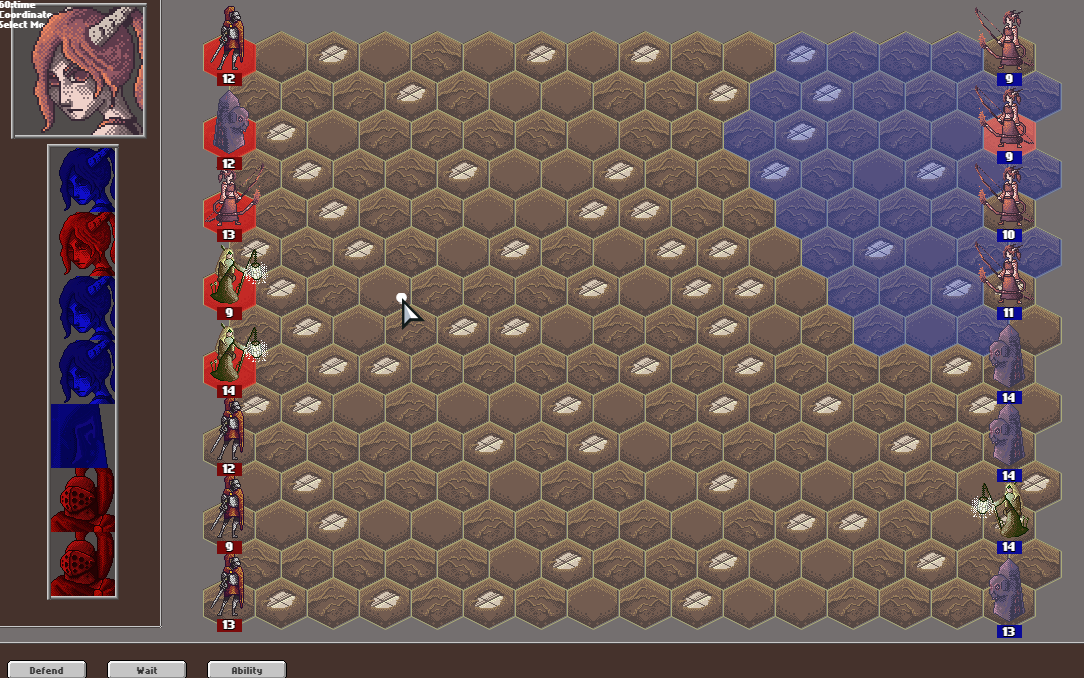
\includegraphics[width=6.2in]{hexmap1.png}
  \caption{Ekran rozgrywki}
  \label{fig:map}
\end{figure}

\subsection{Możliwe akcje}
\begin{itemize}  
\item Ruch 
\par Jednostka może wykorzystać swoja turę na przemieszczanie się pomiędzy swoim aktualnym polem, a polem znajdującym się w zasięgu jej ruchu [Rysunek \ref{fig:moveRange}]. Ruch odbywa się po najkrótszej ścieżce znalezionej pomiędzy danymi polami. Ruch nie może się obyć poza plansze, pole zajęte przez inną jednostkę, pole zajęte przez przeszkodę. Jeżeli jej umiejętność nie definiuje innego sposobu przemieszczania to jednostka nie może przenikać przez inne jednostki oraz przeszkody. Wykorzystanie tej akcji kończy turę. 

\begin{figure}[H]
 \centering
  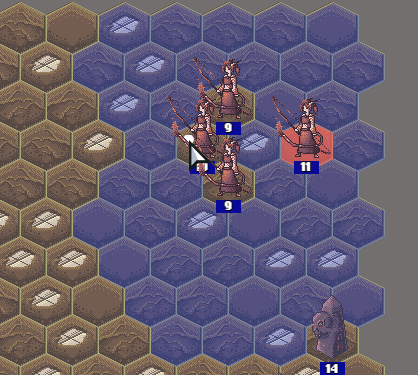
\includegraphics[width=3.2in]{moveRange.png}
  \caption{Zakres ruchu jednostki jest zaznaczony niebieskim kolorem}
  \label{fig:moveRange}
\end{figure}

\item Atak
\par Jeżeli w zasięgu ataku znajduję się jednostka wroga do gracza, może zostać podjęta akcja ataku [Rysunek \ref{fig:attackRange}] (opisane w paragrafie poświęconemu atakowi). Wykorzystanie tej akcji kończy turę. 

\begin{figure}[H]
 \centering
  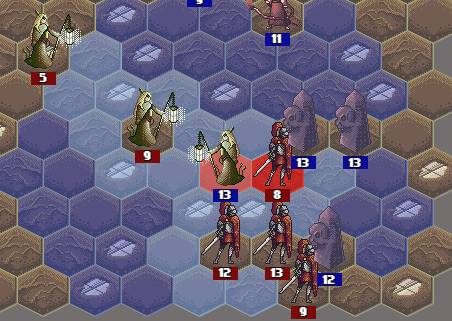
\includegraphics[width=3.2in]{attackRange.png}
  \caption{Możliwe do zaatakowania jednostki są zaznaczone na czerwono}
  \label{fig:attackRange}
\end{figure}

\item Ruch i Atak
\par Jeżeli zasięg jednostki pozwala na przesunięcie tak aby wroga jednostka znajdowała się w zasięgu ataku po poruszeniu obie te akcje można połączyć w jedną.
\item Użycie umiejętności 
\par Niektóre z jednostek posiadają umiejętności które mogą zostać wykorzystane podczas tury danej jednostki  [Rysunek \ref{fig:abilityRange}] (opisane w paragrafie poświęconemu umiejętnością). Wykorzystanie tej akcji kończy turę. 

\begin{figure}[H]
 \centering
  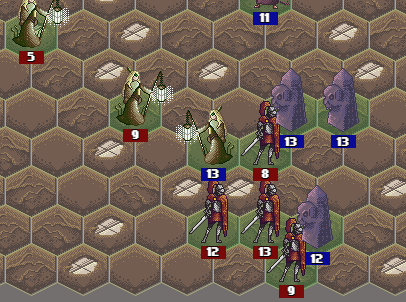
\includegraphics[width=3.2in]{abilityRange.png}
  \caption{Zakres umiejętności jednostki jest zaznaczony zielonym kolorem}
  \label{fig:abilityRange}
\end{figure}

\item Obrona
\par Tura może zostać wykorzystanie do nadania jednostce statu ''Obrona''. Jednostka z tym statusem otrzymuje obrażenia zmniejszone o połowę, aż do swojej następnej tury. Wykorzystanie tej akcji kończy turę. 
\item Czekanie
\par Akcja czekanie przenosi turę jednostki na koniec aktualnej kolejki jednostek. Oznacza to że akcja jednostki zostanie podjęta jeszcze raz podczas tej samej rundy. Akcja ta może zostać wykorzystana raz na rundę (Jeżeli w danej rundzie jednostka czekała nie może czekać jeszcze raz aż do następnej tury) 
\end{itemize}

\subsection{Jednostka}
Każdy z graczy rozpoczynając rozgrywkę posiada zestaw jednostek. Gracz może posiadać wiele jednostek takie samego typu. Jednostki są zorganizowane z grupy. Oznacza to że jednostka reprezentowana pojedyncza postacią na polu walki, tak naprawdę reprezentuje ich wielokrotność [Rysunek \ref{fig:unit}].
\begin{figure}[h!]
 \centering
  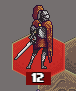
\includegraphics[scale=1.2]{unit.png}
  \caption{Ilość jednostek w grupie jest wyświetlana pod nią}
  \label{fig:unit}
\end{figure}

Jednostki są opisane przez szereg parametrów:
\begin{itemize}  
\item Poziom
\par Poziom jednostki wpływa na silę umiejętności jednostek.
\item Inicjatywa
\par Inicjatywa porządek w którym jednostki wykonują swoje tury. Jednostki o wysokiej inicjatywę poruszającą się wcześniej. Jeżeli jednostki maja taka sama wartość inicjatywy to wybierana jest losowa jednostka. Kolejność jednostek jest ustalana na rozpoczęcie rundy.
\item Punkty życia
\par Punkty życia określają ile obrażeń może przyjąć jednostka zanim zostanie usunięta z pola walki. 
\item Zasięg ataku
\par Ile pól od atakującego może znajdować się przeciwnik, aby dało się go zaatakować bez wykonania ruchu.
\item Punkty obrażeń
Zakres z którego losowane są obrażenia zadawane przez pojedyncza jednostkę.
\item Strzelająca
Jednostka atakuje wręcz czy na odległość.
\item Liczba kontrataków 
Ile razy jednostka może kontratakować w danej rundzie.
\end{itemize}
\subsubsection {Jednostki strzelające}

Jednostki są podzielone ze względu na typ ataku na dwie grupy : atakujące wręcz i strzelające. Strzelcy charakteryzują się zwykle większym zasięgiem ataku, ale jest to związane z pewnymi dodatkowymi efektami. Właściwości jednostek strzelających:

\begin{itemize}
\item Ataki wykonywane na odległość większa niż jedno pole nie skutkują kontratakiem
\item Jeżeli obok znajduje się jednostka przeciwnika, zasięg ataku zostaje zmniejszony do jednego pola
\item Ataki wręcz zadają 50\% obrażeń
\item Po wykonaniu ruchu możliwe jest wykonanie jedynie ataku wręcz (zasięg ataku jest zmniejszony do 1 pola)
\end{itemize}

\subsection{Atak}

Atak może nastąpić jeżeli w zasięgu ataku aktualnej jednostki znajduje się przeciwnik, lub jeżeli znajdzie się tam po wykonaniu ruchu. Atak jest jedynym sposobem na eliminacje jednostek przeciwnika. Atak niszczący jednostkę wroga nie powoduje zmiany pola. Siła ataku jest liczona następująco:
\begin{equation}
attackPower =  p*n + rand(-r*n,r*n)
\end{equation}
Gdzie:
\begin{itemize}
\item p - bazowy atak jednostki
\item n - liczba jednostek
\item r - zmienna losowa ataku jednostki
\end{itemize}

Siła ataku może zostać zmniejszona o 50\% jeżeli atakowany się broni.

\subsubsection {Kontratak}

Jeżeli broniąca się jednostka dalej istnieje, nie przekroczyła ilości kontrataków w danej rundzie, i atakujący nie strzelcem następuje kontratak. Siła kontrataku jest liczona dokładnie w taki sam sposób co atak. Możliwość kontratakowania jest resetowana przy rozpoczęciu tury danej jednostki.

\subsection{Umiejętności}

Jednostki mogą posiadać umiejętności. Na ten moment umiejętności maja jedynie charakter aktywny - są traktowane jako akcja podjęta przez jednostkę podczas jej tury, i ich wykorzystanie ta turę kończy. Każda jednostka może posiadać tylko jedna umiejętność aktywna.
Lista umiejętność : 
\begin{itemize}
\item Leczenie
\par Wybrana jednostka może zostać uleczona. Ilość odnowionych punktów życia nie może przekroczyć utraconej wartości. Jeżeli cała grupa jednostek została zniszczona, nie może zostać ona uleczona. Ilość przywróconych punktów życia jest zależna od ilość jednostek wykorzystując umiejętność oraz ich poziomu.
\item Przyzwanie
\par Na wybranym polu zostaje przyzwana nowa grupa jednostek. Jej tura zaczyna się od nastopnej rundy. Ilość przyzwanych jednostek jest zależna od ilość jednostek wykorzystując umiejętność oraz ich poziomu.
\end{itemize}

\end{document}